\documentclass[11pt,a4paper]{article}
\usepackage[utf8]{inputenc}
\usepackage[spanish]{babel}
\usepackage{amsmath}
\usepackage{amsfonts}
\usepackage{amssymb}
\usepackage{graphicx}
\usepackage{float}
\usepackage{caption}
\captionsetup[table]{name=Tabla}
\setlength{\parindent}{0pt}
\usepackage[left=2cm,right=2cm,top=2cm,bottom=2cm]{geometry}
\author{Marina Esgueva Ruiz}
\begin{document}
\section{Experimentación numérica}
La calidad de las soluciones aproximadas obtenidas con el método de las RBF depende fuertemente de diversos parámetros que influyen en el mismo. Algunos de estos parámetros son la colocación y el número de centros, el tipo de RBF utilizadas como funciones básicas y el parámtro de forma de dichas funciones. Para medir la calidad de las aproximaciones calculadas se utiliza el error cuadrático medio, denotado por ECM, que se calcula de la siguiente forma: 
$$ECM=\sqrt{\frac{1}{M}\sum_{i=1}^M (u(x_i)-s(x_i))^2}$$
donde, \\
$x_1,\ldots,x_M$ son puntos distribuidos en una rejilla uniforme en el dominio, $u$ es la solución real de la EDP y
$s$ es la solución aproximada de la EDP. \\
Los primeros experimentos numéricos se lleva a cabo suponiendo que se conoce la solución real de la EDP. Sin embargo, en la práctica, no disponemos de esta información, por lo que más adelante se definirá una función que estime el error y que pueda ser calculada sin más datos que la ecuación y sus condiciones de frontera. \\
Durante la experimentación numérica trabajamos con las siguientes EDP, definidas en el cuadrado unidad, $\Omega$: 
\begin{equation}
\left \lbrace \begin{array}{cc}
\ \Delta u(x,y)=-\dfrac{5}{4}sin(\pi x) cos(\frac{\pi y}{2}), & (x,y) \in \Omega \\
\ u(x,y)=sin(\pi x), & (x,y)\in \Gamma_1, \\
\ u(x,y)=0, & (x,y) \in \Gamma_2\\ 
\end{array} \right.
\label{edp1}
\end{equation}
donde $\Gamma_1=\lbrace (x,y):0\leq x \leq 1, y=0 \rbrace$ y $\Gamma_2= \partial \Omega \backslash \Gamma_1$.\\
Se puede verificar fácilmente que la solución de la ecuación es: 
$$u(x,y)=sin(\pi x) cos(\frac{\pi y}{2}).$$
\begin{figure}[H]
\centering
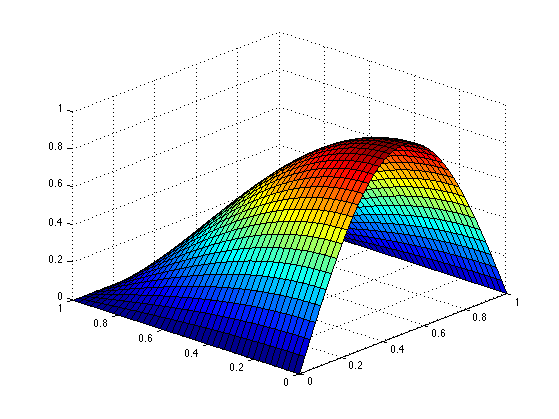
\includegraphics[scale=.5]{u1.png}
\caption{Solución de EDP $(\ref{edp1})$}
\end{figure}
\begin{equation}
\left \lbrace \begin{array}{cc}
\ \Delta u(x,y)=8e^{2x+2y}, & (x,y) \in \Omega\backslash \partial \Omega \\
\ u(x,y)=e^{2x+2y}, & (x,y)\in \partial \Omega, \\
\end{array} \right.
\label{edp 2}
\end{equation}
Es fácil ver que la solución de la ecuación es $e^{2x+2y}$. 
\begin{figure}[H]
\centering
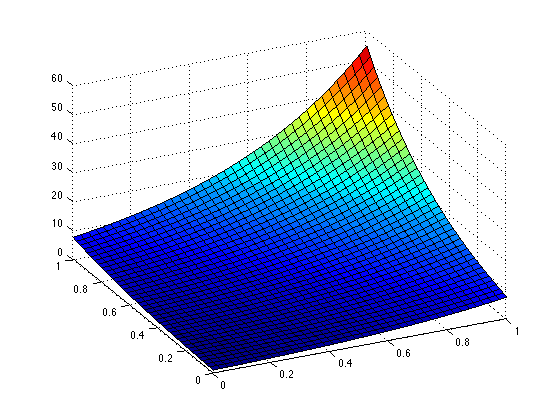
\includegraphics[scale=.5]{u3.png}
\caption{Solución de la EDP $(\ref{edp 2})$}
\end{figure}
\subsection{Distribución y número de centros, tipo de RBF y parámetro de forma.}
En los primeros experimentos llevados a cabo se trabaja con un parámetro de forma fijo, tomando como RBF  multicuádricas inversas y variando el número de centros. Además se diferencia entre colocar todos los centros dentro del dominio o desplazar los centros de la frontera ligeramente fuera del mismo. Para cada una de las aproximaciones obtenidas se recoge el error cometido en la aproximación así como el condicionamiento de la matriz de colocación utilizada. Los centros los distribuimos en una rejilla uniforme en el dominio: 
\begin{figure}[H]
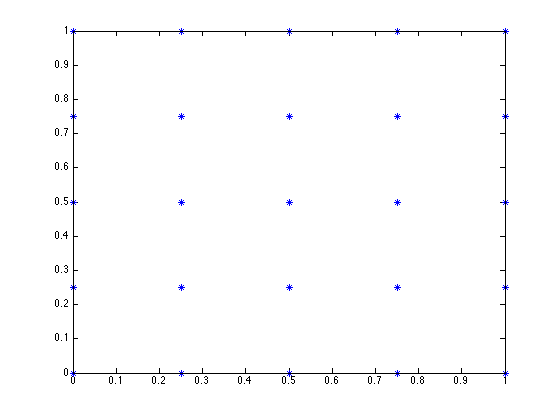
\includegraphics[scale=.4]{distribucion1}
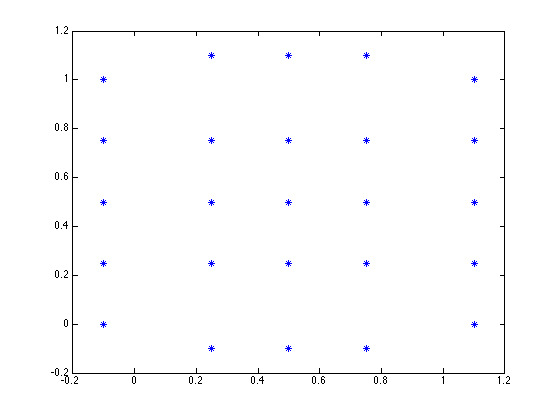
\includegraphics[scale=.4]{distribucion2}
\caption{Distribución de los centros. A la izquierda, todos los centros en el dominio y a la derecha, algunos centros deslplazados fuera del dominio. }
\end{figure} 
\begin{table}[H]
\centering
\caption{$\epsilon=3$. RBF: IMQ. EDP \ref{edp1}}
\begin{tabular}{|c|cc|cc|}
\hline
\ & \multicolumn{2}{|c|}{Centros en la frontera} & \multicolumn{2}{|c|}{Centros fuera del dominio} \\
\hline
\ $N$& ECM & Condicionamiento & ECM & Condicionamiento \\
\hline
\ 9 & 1.55e-01 & 5.55e+01& 1.68e-01 & 6.01e+01 \\
\ 25 &  3.41e-02& 5.76e+02 & 2.40e-02 &6.18e+02  \\
\ 81 & 5.73e-03 & 1.50e+05&  3.28e-03 & 1.27e+05 \\
\ 169 & 1.47e-03 &3.46e+07  & 8.29e-04&1.97e+07  \\
\ 289 &4.17e-04  & 7.64e+09&  2.34e-04&2.99e+09  \\
\ 1089 & 3.69e-06 & 8.37e+19 &   2.15e-06 &5.97e+18  \\
\hline
\end{tabular}
\label{primera comparacion}
\end{table}

\begin{table}[H]
\centering
\caption{$\epsilon=3$. RBF: IMQ. EDP \ref{edp 2}}
\begin{tabular}{|c|cc|cc|}
\hline
\ & \multicolumn{2}{|c|}{Centros en la frontera} & \multicolumn{2}{|c|}{Centros fuera del dominio} \\
\hline
\ $N$& ECM & Condicionamiento & ECM & Condicionamiento \\
\hline
\ 9 & 1.17e-01 & 4.88e+02& 1.28e-01 & 3.77e+02 \\
\ 25 &  1.08e-02& 6.81e+05 & 1.53e-02 &3.75e+05 \\
\ 81 & 2.82e-04 &1.14e+12&  1.32e-03 & 8.76e+11 \\
\ 169 & 4.10e-05 &8.07e+17  &1.07e-03&1.13e+18  \\
\ 289 &5.08e-05  & 2.78e+19&  2.62e-05&1.24e+19  \\
\ 1089 & 9.20e-05 & 5.57e+20 & 1.49e-04 &1.59e+20\\
\hline
\end{tabular}
\label{primera comparacion 2}
\end{table}
En la Tabla \ref{primera comparacion} observamos que aumentar el número de centros mejora la calidad de las soluciones aproximadas. Por el contrario, el condicionamiento de las matrices de colocación aumenta. En todos los casos el error cometido en la aproximación es menor si desplazamos los centros correspondientes a la frontera fuera del dominio. Sin embargo, estas diferencias no son significativas. 
En la Tabla \ref{primera comparacion 2} no siempre disminuye en error al aumentar el número de centros. En algunos casos aumenta aunque no significativamente. En este caso no se cumple que la calidad de la aproximación sea mayor al desplazar los centros fuera del dominio. En algunos casos el error es menor con todos los centros en el dominio y en otros es mayor. \\

En la siguiente tabla comparamos el uso de dos RBF diferentes: la gaussiana y la multicuádrica inversa. Los experimentos se han llevado a cabo fijando el valor del parámetro de forma, $\epsilon=3$, y colocando los centros de la frontera fuera del dominio.  Comparamos el error cometido en la resolución y el condicionamiento de las matrices de colocación utilizando cada uno de los dos tipos de RBF. 
\begin{table}[H]
\centering
\caption{ $\epsilon=3$. Centros fuera del dominio. }
\begin{tabular}{|c|cc|cc|}
\hline
\ & \multicolumn{2}{|c|}{IMQ} & \multicolumn{2}{|c|}{Gaussiana} \\
\hline
\ $N$& ECM & Condicionamiento & ECM & Condicionamiento \\
\hline
\ 9 &   1.68e-01 & 6.01e+01 &2.31e-01&4.81e+01\\
\ 25 &   2.40e-02 &6.18e+02 & 2.17e-02&7.93e+02 \\
\ 81 &   3.28e-03 & 1.27e+05&1.85e-03&1.70e+09 \\
\ 169 &  8.29e-04&1.97e+07&8.85e-05&3.69e+16  \\
\ 289 &  2.34e-04&2.99e+09 &2.20e-06&2.16e+20 \\
\ 1089 & 2.15e-06 &5.97e+18&1.57e-06&  3.86e+20\\
\hline
\end{tabular}
\end{table}
Se observa que las aproximaciones obtenidas utilizando funciones gaussianas cometen un error menor que las que utilizan la multicuádrica inversa. \\
Ahora variamos el parámetro de forma para ver como afecta a la calidad de los resultados. Fijamos 289 centros distribuidos uniformemente en el dominio y medimos el ECM para distintos valores del parámetro de forma $\epsilon$. Además colocamos los centros correspondientes a la frontera fuera del dominio. 

\begin{table}[H]
\centering
\caption{$N=289$.}
\begin{tabular}{|c|cc|cc|}
\hline
\ & \multicolumn{2}{|c|}{IMQ} & \multicolumn{2}{|c|}{Gaussiana} \\
\hline
\ $\epsilon$& ECM & Condicionamiento & ECM & Condicionamiento \\
\hline
\ 1 & 1.59e-06   &2.52e+19  & 7.12e-06& 2.99e+19\\
\ 3 &  2.34e-04  &2.99e+09 & 2.20e-06& 2.16e+20\\
\ 6 &  8.42e-04  & 1.99e+06&  7.41e-04&5.91e+11 \\
\ 9 & 1.47e-03 &2.98e+05& 5.21e-03&1.14e+06  \\
\ 12& 9.76e-03&1.49e+05  & 4.10e-02&7.64e+04 \\

\hline
\end{tabular}
\label{comparacion eps}
\end{table}

Se observa que los errores en la resolución son mayores al aumentar el valor del parámetro de forma. Sin embargo, el condicionamiento de la matriz de colocación sigue la tendencia contraria y es mayor para valores pequeños del parámetro. Por otra parte, al variar el parámetro de forma el error no siempre es menor al utilizar gaussianas como RBF. En algunos caso, la aproximación es mejor utilizando funciones multicuádricas inversas. \\

Como se observa en todo estos experimentos, la calidad de los resultados depende de diferentes aspectos como el número y la distribución de los centros o de parámetro de forma de las RBF. Aumentar el número de centros disminuye el error en la aproximación pero empeora el condicionamiento del problema. Por lo tanto, merece la pena  elegir una colocación óptima de los centros que permita obtener buenos resultados sin utilizar demasiados. Más adelante se definirá un algoritmo con este fin. Por otra parte, también se deben estudiar diferentes estrategias para determinar el parámetro de fórma óptimo. 

\subsection{Reducción de la EDP}
En esta sección se estudia si realizar ciertas modificaciones en la EDP antes de resolverla influye positivamente en la calidad del resultado. Si es posible encontrar una solucion particular bien de las condiciones de frontera o bien de la ecuación, podemos transformar el problema en un problema con condiciones de frontera nulas u homogeneo respectivamente.\\
Si $\tilde{u}$ es una solución particular de la EDP, realizando el cambio de variable $v=u-\tilde{u}$ obtenemos el siguiente problema: 
$$\left \lbrace \begin{array}{cc}
\ \mathcal{L}[v(x,y)]=0 & \text{ si } (x,y) \in \Omega \\
\ v(x,y)=g(x,y)-\tilde{u}(x,y) &  \text{ si } (x,y) \in \partial\Omega \\
\end{array} \right.$$
Si $\hat{u}$ es una función que verifica las condiciones de frontera, realizando el cambio de variable $v=u-\hat{u}$ obtenemos el siguiente problema: 
$$\left \lbrace \begin{array}{cc}
\ \mathcal{L}[v(x,y)]=f(x,y)-\mathcal{L}[\hat{u}(x,y) ]& \text{ si } (x,y) \in \Omega \\
\ v(x,y)=0 & \text{ si } (x,y) \in \partial\Omega \\
\end{array} \right.$$
En caso de que se haya realizado una de estas dos modificaciones, el sistema (añadir referencia) tiene un gran número de ecuaciones homogeneas: las correspondientes al interior o a la frontera. \\

Para estudiar como influyen estas transformaciones del problema en la calidad del resultado, se va a medir el ECM cometido al resolver las ecuaciones \ref{edp1} y \ref{edp 2} de la forma en que aparecen planteadas, transformando la EDP en una ecuación homogénea y transformando las condiciones de frontera. Los experimentos se llevan a cabo fijando el valor del parámetro de forma y se repiten variando el número de centros utilizados en la resolución. Los centros se han colocado dentros del dominio. 

\begin{table}[H]
\centering
\caption{EDP \ref{edp1}. RBF: IMQ. $\epsilon=2$.}
\begin{tabular}{|c|c|c|c|}
\hline
\ $N$ & EDP original & Condiciones de frontera 0 & EDP homogenea \\
\hline
\ 9 & 1.02e-01 & 4.80e-02 & 4.72e-02 \\
\ 25 & 1.29e-02 & 7.93e-03 & 2.10e-02 \\
\ 81 & 1.40e-03 & 1.01e-03& 3.24e-03 \\
\ 169 & 2.09e-04 & 1.68e-04&5.90e-04\\
\ 289 & 3.44e-05&2.934e-05&1.10e-04\\
\ 1089 & 3.35e-07&3.43e-07&1.54e-06\\
\hline  
\end{tabular}
\end{table}



Al transformar el problema en un problema con EDP homogenea se empeoran los resultados obtenidos con el problema original. Si el cambio se realiza para que las condiones de frontera sean nulas, el error es del mismo orden que el obtenido con el problema pero no llega a mejorarlo.  Si repetimos el experimento utilizando funciones gaussianas como RBF obtenemos resultados similares. Una posible explicación al hecho de que transformar la EDP en ecuación homogenea dé tan malos resultados es que al resolver el problema estamos interpolando una función que vale 0 en todo el interior y que toma valores distintos de cero en la frontera y este problema de interpolación presenta grandes dificultades. 


\subsection{Elección del parámetro de forma}
La elección del parámetro de forma adecuado se debe tener en cuenta a la hora de resolver un problema. Hemos visto en la Tabla \ref{comparacion eps}, el ECM varía en varios ordenes de magnitud al emplear diferentes valores del parámetro $\epsilon$. Por lo tanto, se va a describir un algoritmo que permite elegir un parámetro adecuado para la resolución de cada EDP concreta. Desde el punto de vista teórico definimos el parámetro de fórma óptimo de forma óptimo como el valor $\bar{\epsilon}$ que verifica:
$$\bar{\epsilon}=\displaystyle\min_{\epsilon\in \mathbb{R}} ECM(\epsilon).$$
Sin embargo, en la práctica no es posible calcular el ECM ya que no disponemos de la solución de la EDP. Con el objetivo de poder determinar en la práctica un parámetro de forma adecuado vamos a definir una función que, dados los centros y el parámetro de forme, proporcione una estimación del ECM. Llamaremos a esta función $\overline{ECM(\epsilon)}$ y elegimos como óptimo el valor de $\tilde{\epsilon}$ verificando 
$$\bar{\epsilon}=\displaystyle\min_{\epsilon\in \mathbb{R}} \overline{ECM}(\epsilon).$$
Para definir la función $\tilde{ECM}$ aprovechamos que se conoce el valor de la función en la frontera y el del término fuente en el interior del dominio. Tomamos $M$ suficientemente grande y definimos una rejiilla uniforme de $M$ puntos. Dividimos estos puntos en dos conjuntos: $\lbrace x_1,\ldots,x_{m_i}\rbrace$ son los puntos de la rejilla que están en el interior del dominio y $\lbrace y_1,\ldots,y_{m_b}\rbrace$ son los puntos de la rejilla de la frontera. Definimos $\overline{ECM}$ como: 
$$\overline{ECM}(\epsilon)=\sqrt{\frac{1}{M}\left[ \displaystyle \sum_{i=1}^{n_i} (u(x_i)-\hat{u}_\epsilon (x_i))^2+\displaystyle \sum_{i=1}^{n_b} (u(y_i)-\hat{u}_\epsilon (y_i))^2\right]}$$
A continuación, se comprueba que la función $\overline{ECM}$ es realmente un buen estimador del ECM. Para ello representamos ambas funciones conjuntamente para algunos ejemplos de los que se conoce la solución. Variamos el número de centros utilizados en las aproximaciones y variamos también el tipo de RBF utilizado. La curva roja se corresponde con la estimación del error y la azul al ECM real. 
\begin{figure}[H]
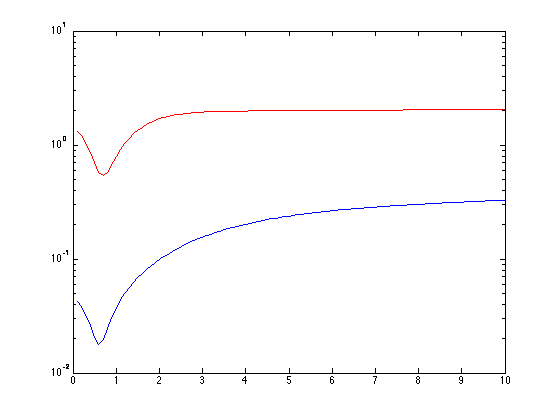
\includegraphics[scale=.45]{est_1_9_imq.png}
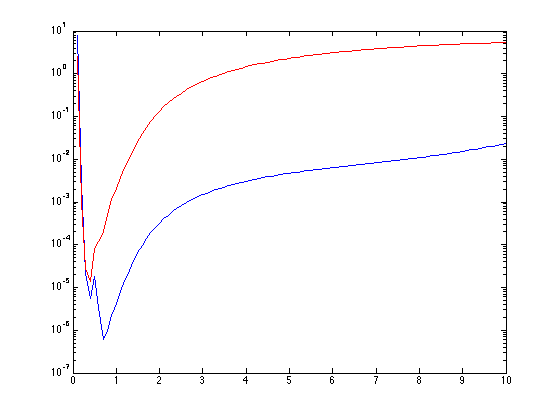
\includegraphics[scale=.45]{est_1_169_imq.png}
\caption{ECM y $\overline{ECM}$ para la EDP \ref{edp1}. RBF: IMQ. $N=9,160$ (de izquierda a derecha)}
\label{estimacion1}
\end{figure}
\begin{figure}[H]
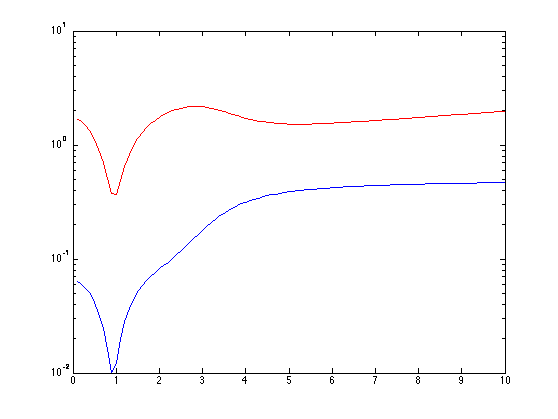
\includegraphics[scale=.45]{est_1_9_gauss.png}
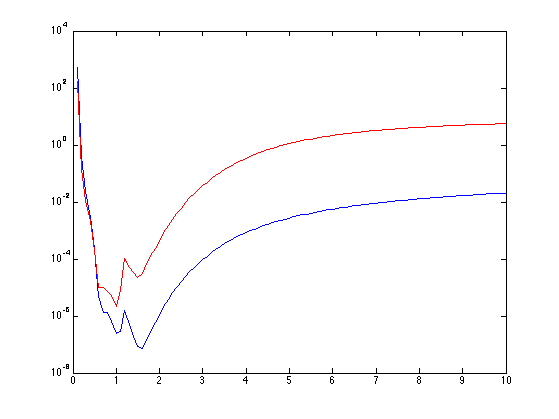
\includegraphics[scale=.45]{est_1_169_gauss.png}
\caption{ECM y $\overline{ECM}$ para la EDP \ref{edp1}. RBF: gaussiana. $N=9,160$ (de izquierda a derecha)}
\label{estimacion2}
\end{figure}
En las Figuras \ref{estimacion1} y \ref{estimacion2} se observa que La función $\overline{ECM}$ sobreestima el ECM. Sin embargo, tiene el mismo perfil que el ECM y alcanzan el mínimo en el mismo punto. Por lo tanto, es adecuada para determinar el parámetro de forma óptimo. Repitiendo los mismos experimentos con otras EDP's se obtienen el mismo resultado. En la siguiente tabla comparamos el valor óptimo del parámetro de forma con el estimado y los errores que se cometen tomando como parámetros el óptimo o el estimado. 
\begin{table}[H]
\centering
\caption{Comparación del parámetro óptimo con el parámetro estimado. RBF: multicuádrica inversa.}
\centering
\begin{tabular}{|c|cccc|}
\hline
$N$ & $\epsilon$ &$ECM(\epsilon)$ & $\bar{\epsilon}$ & $ECM(\bar{\epsilon})$ \\
\hline
9 & 6.09e-01 & 1.78e-02 & 6.97e-01 & 1.95e-02 \\
25 & 2.93e-01&1.34e-04& 2.90e-01& 1.36e-04\\
81 & 4.39e-01&1.05e-06&4.08e-01&1.54e-06\\
169 & 6.53e-01&2.52e-07& 9.63e-01&3.35e-06\\
289&1.05 & 2.67e-07& 9.02e-01 & 3.36e-07\\
1089 & 2.44 & 4.44e-07 & 9.93e-01& 1.04e-06\\
\hline
\end{tabular}
\end{table}
Observamos que a medida que aumenta el número de centros, los valores estimados para $\epsilon$ se alejan más del óptimo, sobre todo en los casos $N=169 $ y $N=1089$. Para el resto de los casos, los valores estimados son cercanos al óptimo y el error cometido utilizando el valor estimado es similar al cometido con el óptimo. 
\section{Parámetro de forma variable}
La elección del parámetro de forma tiene gran influencia en la calidad de los resultados, como hemos comprorado en los experimentos previos. Por lo tanto, además de la elección óptima del parámetro $\epsilon$, se pueden llevar a cabo otras estrategias con el objetivo de mejorar la calidad del resultado. En (añadir referencias) se introduce la idea de tomar valores diferentes del parámetro de forma para los diferentes centros, es decir que el aproximante $\hat{u}$ tenga la forma: 
$$\hat{u}(x)=\displaystyle \sum_{i=1}^N \alpha_i \varphi_{\epsilon_i}(||x-c_i||)$$
Ahora los valores $\epsilon_i$ asociados a cada uno de los centros pueden ser diferentes. Al variar el parámetro de forma asociado a cada centro, se pierde cualquier simetria o estructura especial en las matrices de colocación. Sin embargo, estas diferencias entre las entradas pueden conducir a una disminución del condicionamiento de las mismas. \\
Se han llevado a cabo experimentos numéricos para verificar la eficacia del uso de un parámetro de forma variable. En primer  lugar, utilizamos unicamente dos valores diferentes de $\epsilon$: uno asociado a los centros del interior del dominio y otro a los de su frontera.  Comenzamos seleccionando el parámetro de forma óptimo para todo el dominio y lo fijamos en el interior, calculando el óptimo para la frontera, teniendo en cuenta que debe ser menor que en interior. Los resultados obtenidos son los siguientes: 

\begin{table}[H]

\centering
\caption{Elección óptima del parámetro de forma para la EDP \ref{edp1}. RBF: multicuádrica inversa.}
\begin{tabular}{|c|ccc|}
\hline
\ $N$ & $\epsilon$ & ECM & Condicionamiento \\
\hline
\ 9 & 6.97e-01 & 1.95e-02 & 3.45e+03 \\
\ 25 & 2.89e-01 & 1.36e-04 & 6.64e+12\\
\ 81&4.08e-01 & 1.54e-06 & 7.17e+18\\
\ 169 & 9.63e-01 & 3.35e-06& 5.36e+17\\
\ 289 & 9.02e-01& 3.37e-07 & 4.11e+19\\
\ 1089 & 9.92e-01 &1.03e-06 & 1.71e+20 \\
\hline
\end{tabular}
\label{ep_optimo}
\end{table}


\begin{table}[H]

\centering
\caption{Elección óptima del parámetro de forma para la EDP \ref{edp1} distinguiendo entre interior y frontera. RBF: multicuádrica inversa.}
\begin{tabular}{|c|cccc|}
\hline
\ $N$ & $\epsilon$ interior &$\epsilon$ frontera&ECM & Condicionamiento \\
\hline
\ 9 & 6.97e-01 & 6.80e-01& 1.86e-02 &3.94e+03 \\
\ 25 & 2.89e-01 &2.61e-01& 1.01e-03 &9.38e+10\\
\ 81& 4.08e-01 &3.26e-01&7.40e-07& 2.54e+18\\
\ 169 & 9.63e-01&5.81e-01 & 6.68e-07& 4.23e+18\\
\ 289 & 9.02e-01& 6.71e-01& 5.95e-08 & 9.11e+18\\
\ 1089 & 9.92e-01&2.94e-01& 4.73e-07 &5.73e+20 \\
\hline

\end{tabular}
\label{ep_variable}
\end{table}
Al comparar las Tablas \ref{ep_optimo} y \ref{ep_variable} se puede comprobar que, excepto en el caso $N=25$, la calidad de las soluciones obtenidas es mayor si distinguimos el valor del parámetro de forma en el interior y en la frontera. Cuando se trabaja con un número reducido de centros las diferencias en el error que comenten cada una de las estrategias en menor, pero a partir de 81 centros estas diferencias son bastantes significativas. En cuanto al condicionamiento, no se aprecia que la introducción del parámetro de forma variable suponga una disminución del mismo. 

En (añadir referecia Sarra) introducen algunas otras estrategias en las que cada centro tiene asociado un parámetro de forma diferente. $\epsilon$ se puede determinar con expresiones como las siguientes:
\begin{equation}
\epsilon_j=\bar{\epsilon}\dfrac{1}{\sqrt{1+K(-1)^j}}
\label{estrategia1}
\end{equation}
\begin{equation}
\epsilon_j=\sqrt{\epsilon_{min}^2\frac{\epsilon_{max}^2}{\epsilon_{min}^2}^\frac{j-1}{N-1}}
\label{estrategia 2}
\end{equation}
En \ref{estrategia1} el parámetro de forma varía alrededor del valor $\bar{\epsilon}$, que es el parámetro de forma óptimo para el problema. En \ref{estrategia 2} el parámetro varía entre unos valores máximos y mínimos: $\epsilon_{max}$ y $\epsilon_{min}$. En ambas estrategias, el parámetro de forma elegido para cada centro depende de la numeración de los centros. En la primera de las estrategias, el parámetro solo toma dos valores en función de si un centro es par o impar de acuerdo a la numeración elegida. Con la segunda estrategia se elige un valor diferente para cada centro pero, nuevamente, cambiar la numeración de los centros modifica la asignación de parámetros de forma. Para asignar un parámetro diferente a cada centro, parece más adecuado utilizar algun método aleatorio en el que no influya el órden de los centros. Una posible estrategia es asignar valores aleatorios de acuerdo a una distribución uniforme entre dos valores máximo y mínimo:
\begin{equation}
\label{estrategia 3}
\epsilon=\epsilon_{min}+(\epsilon_{max}-\epsilon_{min})\times u,
\end{equation} 
donde $u$ sigue una distribución uniforme en el intervalo $(0,1)$. \\
 Alternativamente, se pueden determinar los parámetros óptimos para los centros del interior y para los de la frontera y elegir aleatoriamente un valor de $\epsilon$ alrededor de la media correspondiente.
\begin{equation}
\label{estrategia 4}
\epsilon=\bar{\epsilon}\times (0.5+u) 
\end{equation}
donde $u$ sigue una distribución uniforme en el intervalo $(0,1)$.\\

\begin{table}[H]
\centering
\caption{Estrategias aleatorias de elección de $\epsilon$. RBF: multicuádrica inversa. EDP \ref{edp1} }
\centering
\begin{tabular}{|c|cc|cc|}
\hline
\ $N$ &\multicolumn{2}{|c|}{Estrategia \ref{estrategia 3}}& \multicolumn{2}{|c|}{Estrategia \ref{estrategia 4}} \\
\hline
\  & ECM & Condicionamiento & ECM & Condicionamiento \\
\hline
\ 9 & 7.97e-02 & 1.24e+03 & 6.29e-02 & 2.84e+03\\
\ 25 & 4.58e-02 & 4.21e+06 & 3.94e-03 & 1.63e+09\\
\ 81 & 2.05e-04& 3.09e+12 &   3.88e-05 & 1.31e+18 \\
\ 169 & 1.82e-05 & 4.09e+17 & 2.74e-07 & 1.14e+19\\
\ 289 & 7.14e-08 & 5.30e+18 & 3.99e-08 & 5.76e+18\\
\ 1089 & 1.29e-10 & 1.78e+21 & 7.67e-10 & 1.46e+20\\
\hline

\end{tabular}
\label{eps aleatorio}
\end{table}
 Al comparar las Tablas \ref{ep_variable} y \ref{eps aleatorio}, se observa que las técnicas aleatorias para la elección del parámetro de forma proporcionan muy buenos resultados. Cuando se utilizan muchos centros para resolver la EDP (más de 200), el ECM del aproximante de la solución es menor si seguimos una estrategia aleatoria para la elección de $\epsilon$. Sin embargo, cuando trabajamos con un número menor de centros, todas las estrategias proporcionan resultados de calidad similar. 
\end{document}